\begin{figure*}[t]
\begin{minipage}{0.5\linewidth}
  \centering
        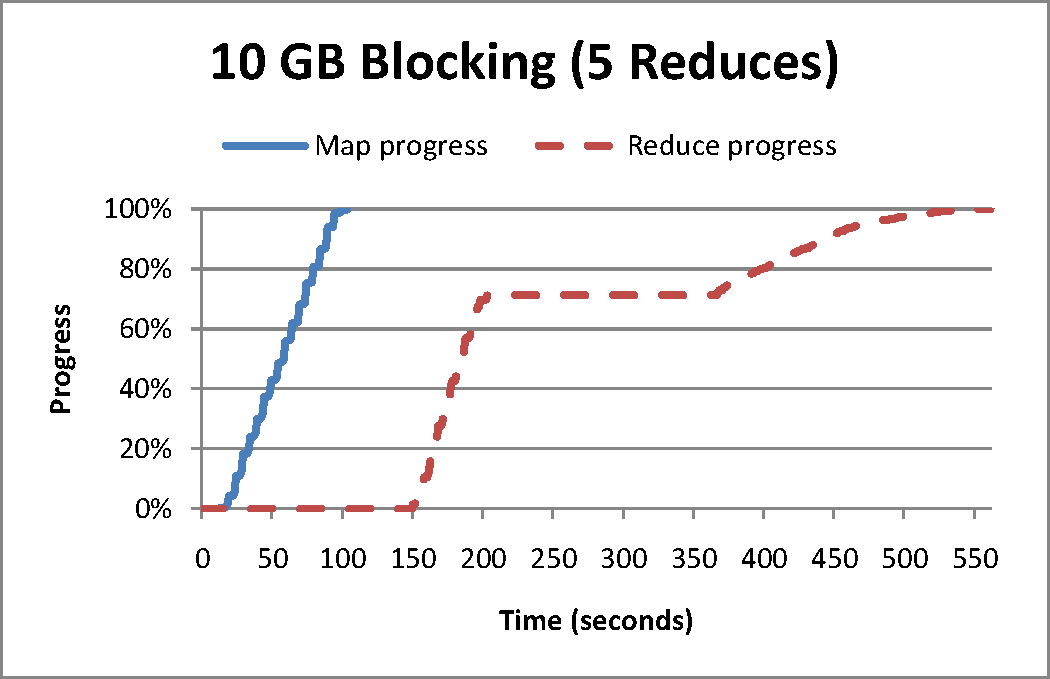
\includegraphics[width=0.90\linewidth]{eval/wc_10gb_20m5r_blocking}
\end{minipage}
\begin{minipage}{0.5\linewidth}
  \centering
        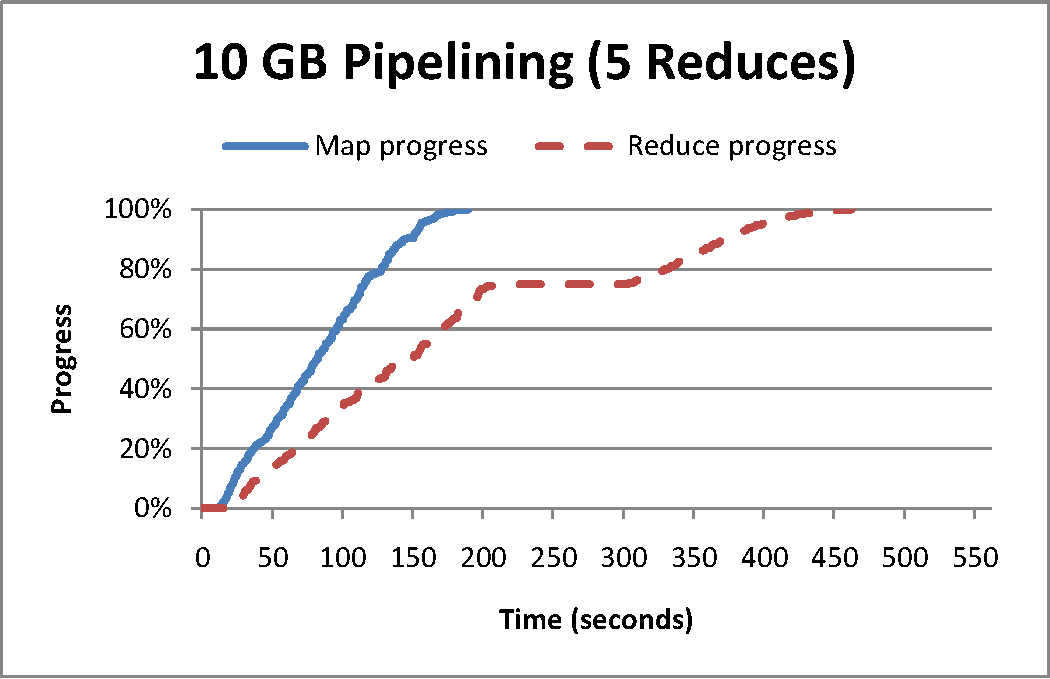
\includegraphics[width=0.90\linewidth]{eval/wc_10gb_20m5r_pipeline}
\end{minipage}
\caption{CDF of map and reduce task completion times for a 10GB wordcount job
  using 20 map tasks and 5 reduce tasks (512MB block size). The total job
  runtimes were 561 seconds for blocking and 462 seconds for pipelining.}
\label{fig:wc1}
\vspace{-4pt}
\end{figure*}

\begin{figure*}[t]
\begin{minipage}{0.5\linewidth}
  \centering
        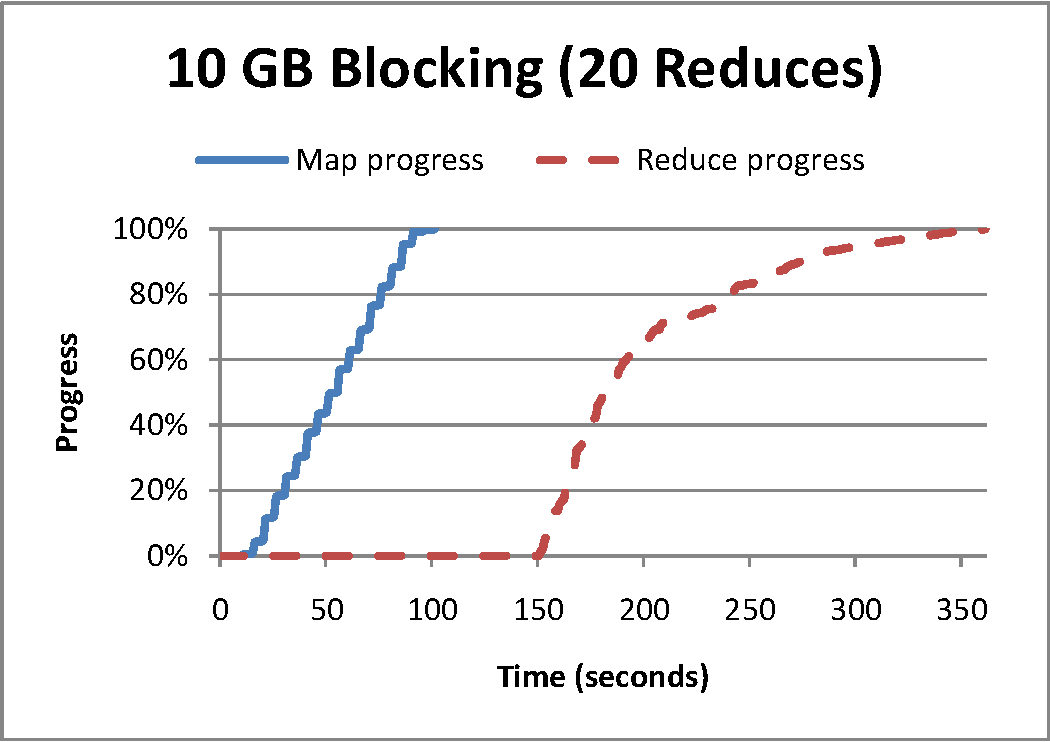
\includegraphics[width=0.88\linewidth]{eval/wc_10gb_20m20r_blocking}
\end{minipage}
\begin{minipage}{0.5\linewidth}
  \centering
        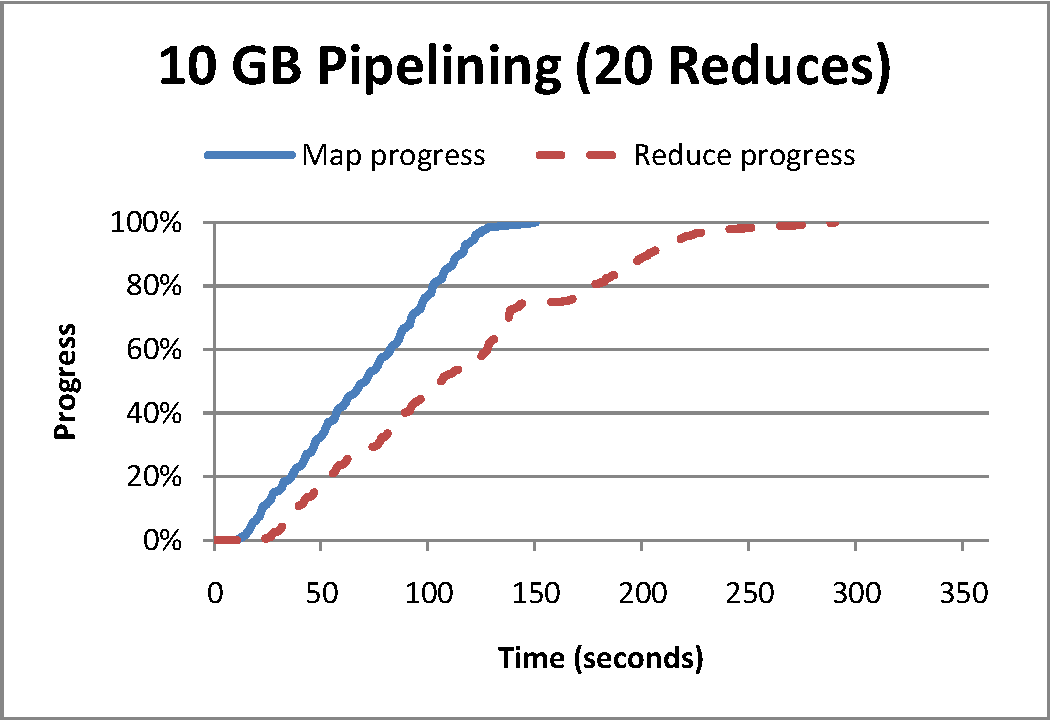
\includegraphics[width=0.90\linewidth]{eval/wc_10gb_20m20r_pipeline}
\end{minipage}
\caption{CDF of map and reduce task completion times for a 10GB wordcount job
  using 20 map tasks and 20 reduce tasks (512MB block size). The total job
  runtimes were 361 seconds for blocking and 290 seconds for pipelining.}
\label{fig:wc2}
\vspace{-4pt}
\end{figure*}

\begin{figure*}[t]
\begin{minipage}{0.5\linewidth}
  \centering
        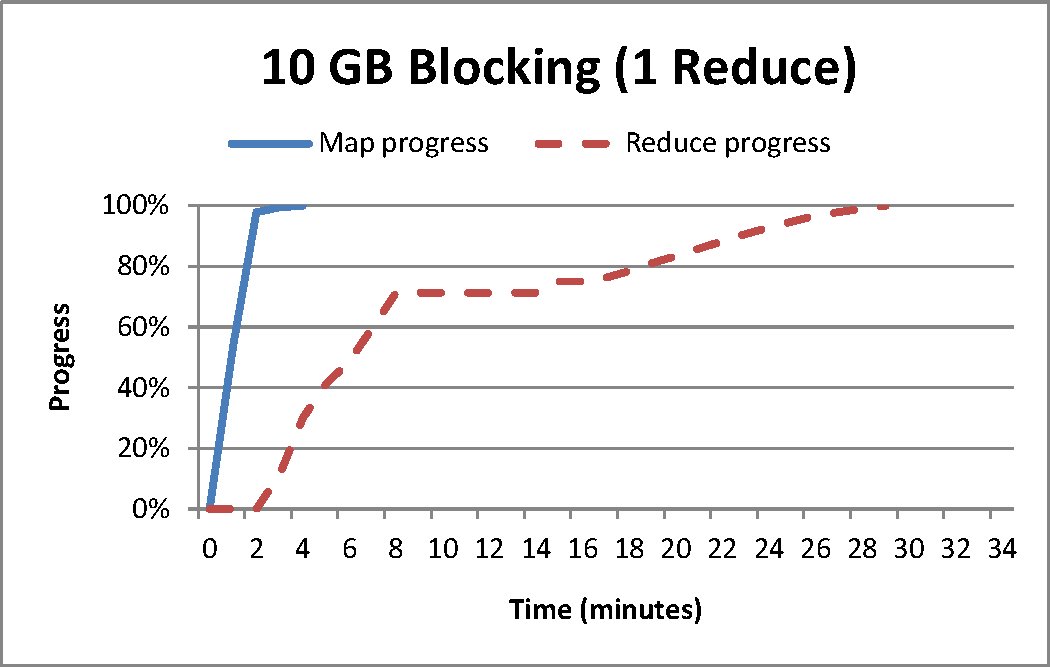
\includegraphics[width=0.95\linewidth]{eval/wc_10gb_20m1r_blocking}
\end{minipage}
\begin{minipage}{0.5\linewidth}
  \centering
        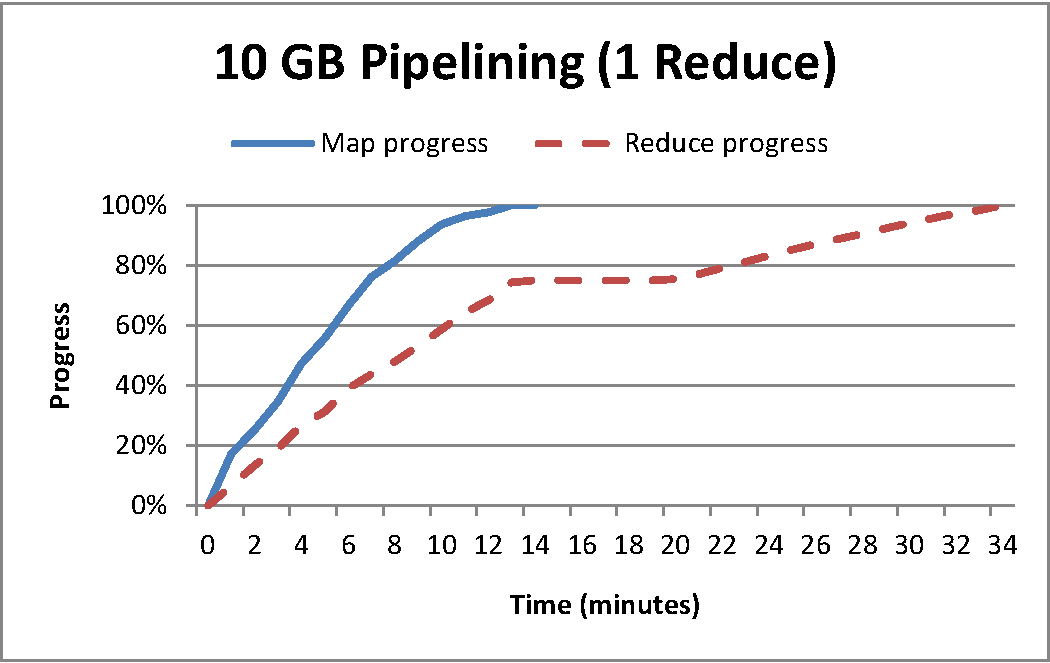
\includegraphics[width=0.95\linewidth]{eval/wc_10gb_20m1r_pipeline}
\end{minipage}
\caption{CDF of map and reduce task completion times for a 10GB wordcount job
  using 20 map tasks and 1 reduce task (512MB block size). The total job
  runtimes were 29 minutes for blocking and 34 minutes for pipelining.}
\label{fig:wc3}
\vspace{-4pt}
\end{figure*}

\section{Performance Evaluation}
\label{sec:perf}

A thorough performance comparison between pipelining and blocking is beyond the
scope of this paper. In this section, we instead demonstrate that pipelining can
reduce job completion times in some configurations.

We report performance using both large (512MB) and small (32MB) HDFS block sizes
using a single workload (a wordcount job over randomly-generated text). Since
the words were generated using a uniform distribution, map-side combiners were
ineffective for this workload. We performed all experiments using relatively
small clusters of Amazon EC2 nodes. We also did not consider performance in an
environment where multiple concurrent jobs are executing simultaneously.

\begin{figure*}[t]
\begin{minipage}{0.5\linewidth}
  \centering
        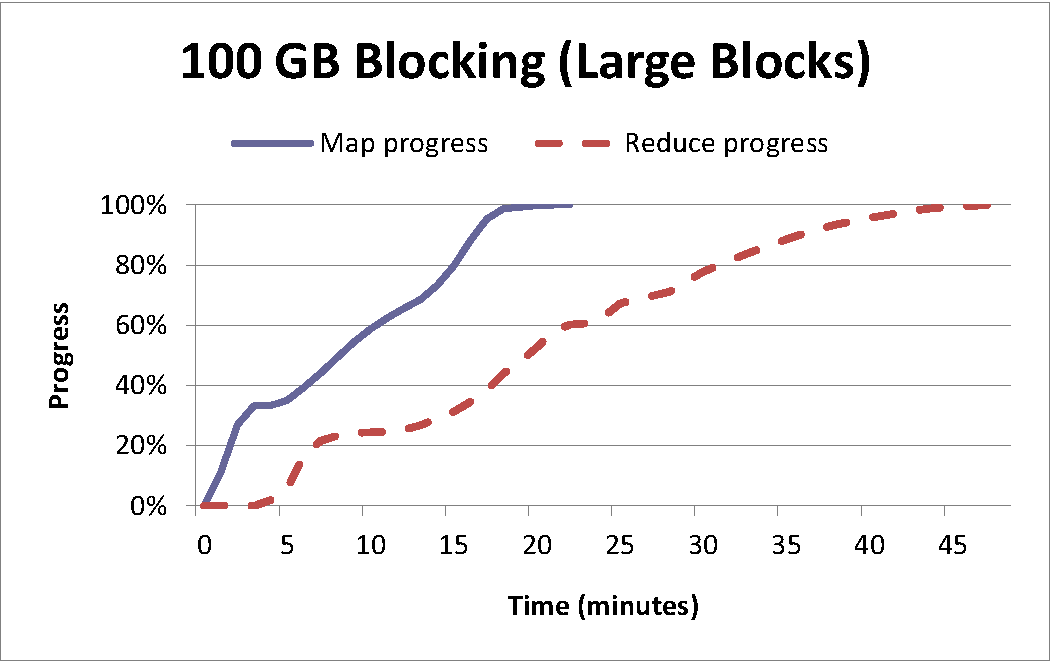
\includegraphics[width=0.95\linewidth]{eval/wc_100gb_240m60r_blocking}
\end{minipage}
\begin{minipage}{0.5\linewidth}
  \centering
        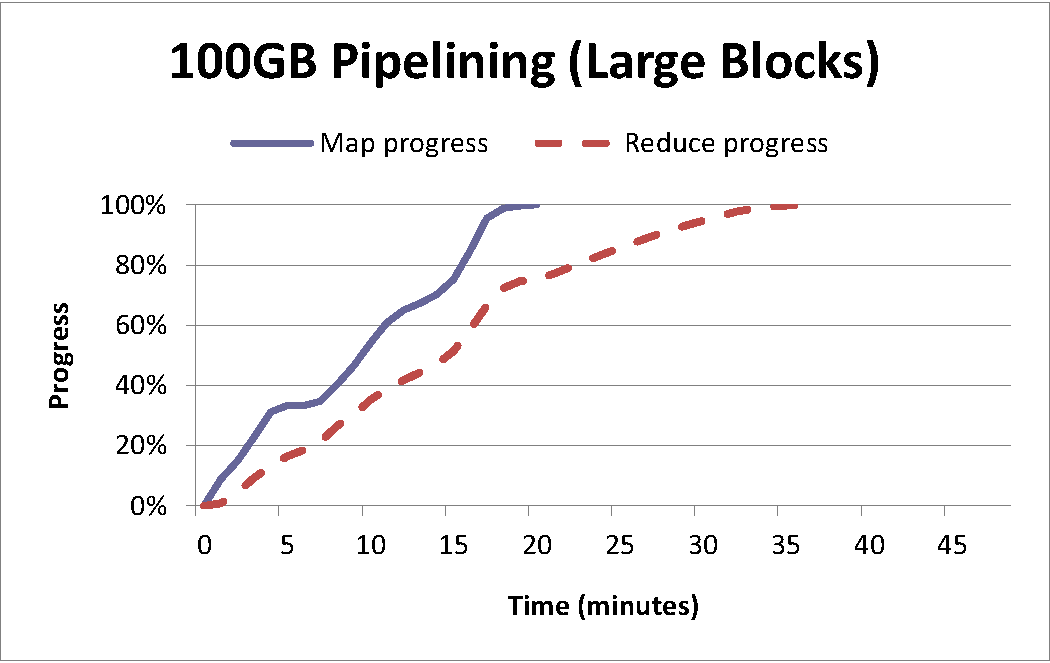
\includegraphics[width=0.95\linewidth]{eval/wc_100gb_240m60r_pipeline}
\end{minipage}
\caption{CDF of map and reduce task completion times for a 100GB wordcount job
  using 240 map tasks and 60 reduce tasks (512MB block size). The total job
  runtimes were 48 minutes for blocking and 36 minutes for pipelining.}
\label{fig:wc4}
\end{figure*}

\begin{figure*}[t]
\begin{minipage}{0.5\linewidth}
  \centering
        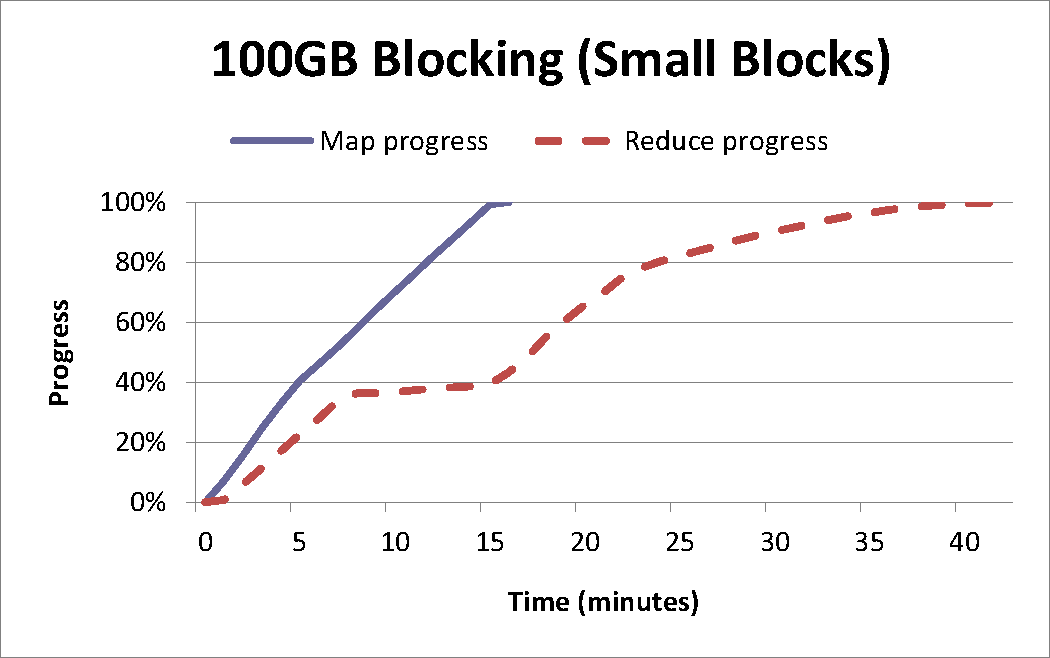
\includegraphics[width=0.95\linewidth]{eval/wc_100gb_3120m60r_blocking}
\end{minipage}
\begin{minipage}{0.5\linewidth}
  \centering
        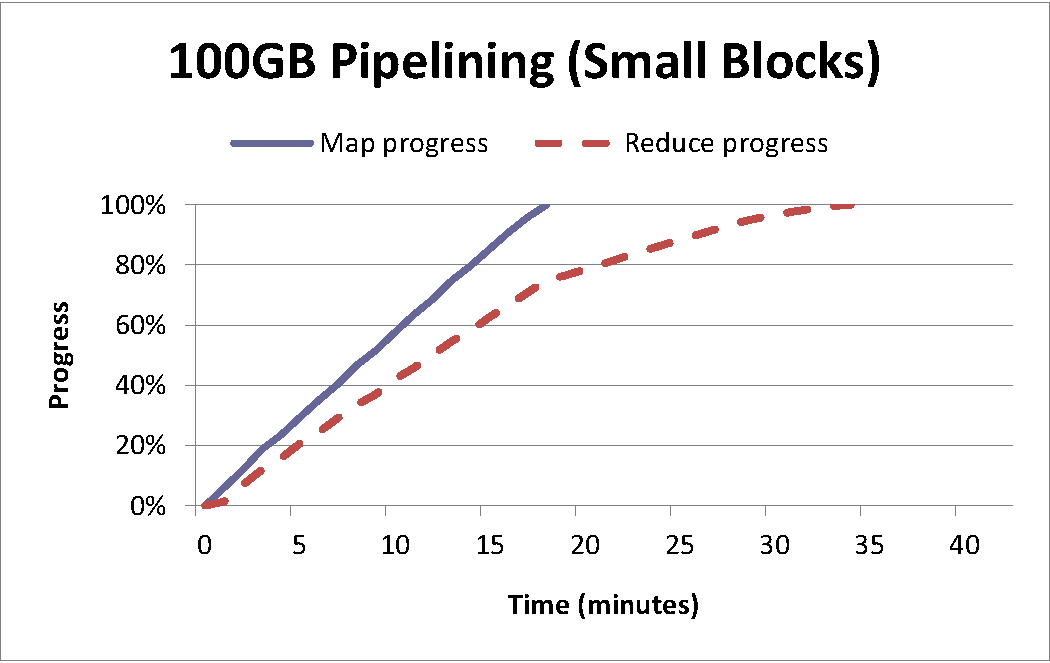
\includegraphics[width=0.95\linewidth]{eval/wc_100gb_3120m60r_pipeline}
\end{minipage}
\caption{CDF of map and reduce task completion times for a 100GB wordcount job
  using 3120 map tasks and 60 reduce tasks (32MB block size). The total job
  runtimes were 42 minutes for blocking and 34 minutes for pipelining.}
\label{fig:wc5}
\end{figure*}

\subsection{Background and Configuration}
Before diving into the performance experiments, it is important to further
describe the division of labor in a HOP job, which is broken into task phases. A
map task consists of two work phases: {\em map} and {\em sort}. The majority
of work is performed in the {\em map} phase, where the map function is applied
to each record in the input and subsequently sent to an output buffer.  Once the
entire input has been processed, the map task enters the {\em sort} phase, where
a final merge sort of all intermediate spill files is performed before
registering the final output with the \TT. The progress reported by a map task
corresponds to the {\em map} phase only.

A reduce task in HOP is divided into three work phases: {\em shuffle}, {\em
  reduce}, and {\em commit}.  In the {\em shuffle} phase, reduce tasks receive
their portion of the output from each map.  In HOP, the {\em shuffle} phase
consumes 75\% of the overall reduce task progress while the remaining 25\% is
allocated to the {\em reduce} and {\em commit} phase.\footnote{The stock version
  of Hadoop divides the reduce progress evenly among the three phases. We
  deviated from this approach because we wanted to focus more on the progress
  during the {\em shuffle} phase.}  In the {\em shuffle} phase, reduce tasks
periodically perform a merge sort on the already received map output. These
intermediate merge sorts decrease the amount of sorting work performed at the
end of the {\em shuffle} phase. After receiving its portion of data from all map
tasks, the reduce task performs a final merge sort and enters the {\em reduce}
phase.

By pushing work from map tasks to reduce tasks more aggressively, pipelining can
enable better overlapping of map and reduce computation, especially when the
node on which a reduce task is scheduled would otherwise be
underutilized. However, when reduce tasks are already the bottleneck, pipelining
offers fewer performance benefits, and may even hurt performance by placing
additional load on the reduce nodes.

The {\em sort} phase in the map task minimizes the merging work that reduce
tasks must perform at the end of the {\em shuffle} phase. When pipelining is
enabled, the {\em sort} phase is avoided since map tasks have already sent some
fraction of the spill files to concurrently running reduce tasks. Therefore,
pipelining increases the merging workload placed on the reducer. The adaptive
pipelining scheme described in Section~\ref{sec:mapout} attempts to ensure that
reduce tasks are not overwhelmed with additional load.

We used two Amazon EC2 clusters depending on the size of the experiment:
``small'' jobs used 10 worker nodes, while ``large'' jobs used 20. Each node
was an ``extra large'' EC2 instances with 15GB of memory and four virtual cores.

\subsection{Small Job Results}
Our first experiment focused on the performance of small jobs in an
underutilized cluster. We ran a 10GB wordcount with a 512MB block size, yielding
20 map tasks. We used 10 worker nodes and configured each worker to execute at
most two map and two reduce tasks simultaneously. We ran several experiments to
compare the performance of blocking and pipelining using different numbers of
reduce tasks.

Figure~\ref{fig:wc1} reports the results with five reduce tasks. A plateau can
be seen at 75\% progress for both blocking and pipelining. At this point in the
job, all reduce tasks have completed the {\em shuffle} phase; the plateau is
caused by the time taken to perform a final merge of all map output before
entering the {\em reduce} phase. Notice that the plateau for the pipelining case
is shorter. With pipelining, reduce tasks receive map outputs earlier and can
begin sorting earlier, thereby reducing the time required for the final merge.

Figure~\ref{fig:wc2} reports the results with twenty reduce tasks. Using more
reduce tasks decreases the amount of merging that any one reduce task must
perform, which reduces the duration of the plateau at 75\% progress. In the
blocking case, the plateau is practically gone.%  However, with pipelining we
% still see a small plateau at 75\%, which means that the final sort spilled to
% disk. Since the combiner is not executed on the full map output, pipelining can
% add extra memory pressure over blocking. That extra memory pressure for this
% experiment was not enough slow pipelining down over blocking. However, a job
% that contains a more effective combiner may be better executed in blocking
% mode.

Note that in both experiments, the map phase finishes faster with blocking than
with pipelining. This is because pipelining allows reduce tasks to begin
executing more quickly; hence, the reduce tasks compete for resources with the
map tasks, causing the map phase to take slightly longer. In this case, the
increase in map duration is outweighed by the increase in cluster utilization,
resulting in shorter job completion times: pipelining reduced completion time by
17.7\% with 5 reducers and by 19.7\% with 20 reducers.

Figure~\ref{fig:wc3} describes an experiment in which we ran a 10GB wordcount
job using a single reduce task. This caused job completion times to increase
dramatically for both pipelining and blocking, because of the extreme load
placed on the reduce node. Pipelining delayed job completion by
\texttildelow{}17\%, which suggests that our simple adaptive flow control scheme
(Section~\ref{sec:mapout}) was unable to move load back to the map tasks
aggressively enough.

\subsection{Large Job Results}
Our second set of experiments focused on the performance of somewhat larger
jobs. We increased the input size to 100GB (from 10GB) and the number of worker
nodes to 20 (from 10). Each worker was configured to execute at most four map
and three reduce tasks, which meant that at most 80 map and 60 reduce tasks
could execute at once. We conducted two sets of experimental runs, each run
comparing blocking to pipelining using either large (512MB) or small (32MB)
block sizes. We were interested in blocking performance with small block sizes
because blocking can effectively emulate pipelining if the block size is small
enough.

Figure~\ref{fig:wc4} reports the performance of a 100GB wordcount job with 512MB
blocks, which resulted in 240 map tasks, scheduled in three waves of 80 tasks
each. The 60 reduce tasks were coscheduled with the first wave of map tasks. In
the blocking case, the reduce tasks began working as soon as they received the
output of the first wave, which is why the reduce progress begins to climb
around four minutes (well before the completion of all maps). Pipelining was
able to achieve significantly better cluster utilization, and hence reduced job
completion time by \texttildelow{}25\%.

% Comparing the reduce progress in blocking to pipelining, we see that reduce
% tasks make more progress during the {\em shuffle} phase when pipelining is
% enabled. What is even more interesting is that the {\em reduce} phase is also
% shorter in the case of pipelining. The reason for this is subtle; all reduce
% tasks enter the {\em phase} around the same time since data is shipped in
% smaller increments. In the blocking case, when the final wave of map tasks
% finish they all try to send the entire output to reduce tasks at the same time,
% which increases the variance on receiving the complete output from all map
% tasks. That is, some reduce tasks enter the {\em reduce} phase well in advance
% of others.

Figure~\ref{fig:wc5} reports the performance of blocking and pipelining using
32MB blocks. While the performance of pipelining remained similar, the
performance of blocking improved considerably, but still trailed somewhat behind
pipelining. Using block sizes smaller than 32MB did not yield a significant
performance improvement in our experiments.

% \subsection{Discussion}

% As mentioned before, a complete performance evaluation is beyond the scope for this paper and we leave
% such a study for future work. The focus here was to provide some initial insight into the performance benefits
% of pipelining. We also wanted to evaluate the adaptive policy of our pipelining scheme. To this end, we
% found such a policy paramount in discovering the right amount of pipelining to perform based on runtime
% factors; network capacity and reduce task (consumer) load.

%\begin{figure*}[t]
%\begin{minipage}{0.5\linewidth}
%        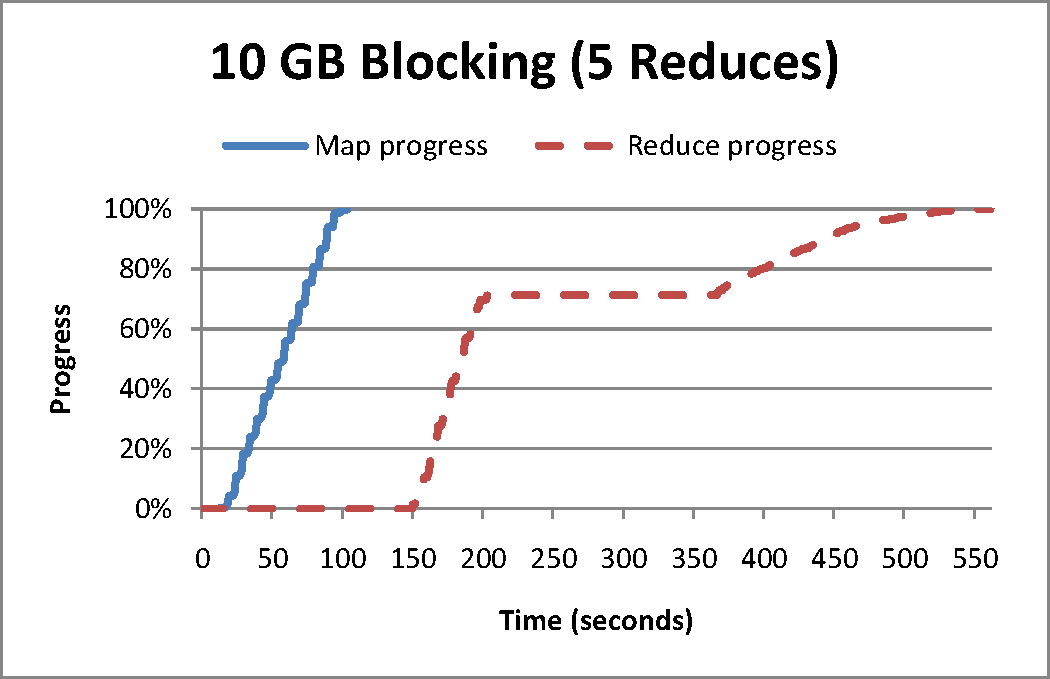
\includegraphics[width=0.95\linewidth]{eval/wc_10gb_20m5r_blocking}
%\end{minipage}
%\begin{minipage}{0.5\linewidth}
%        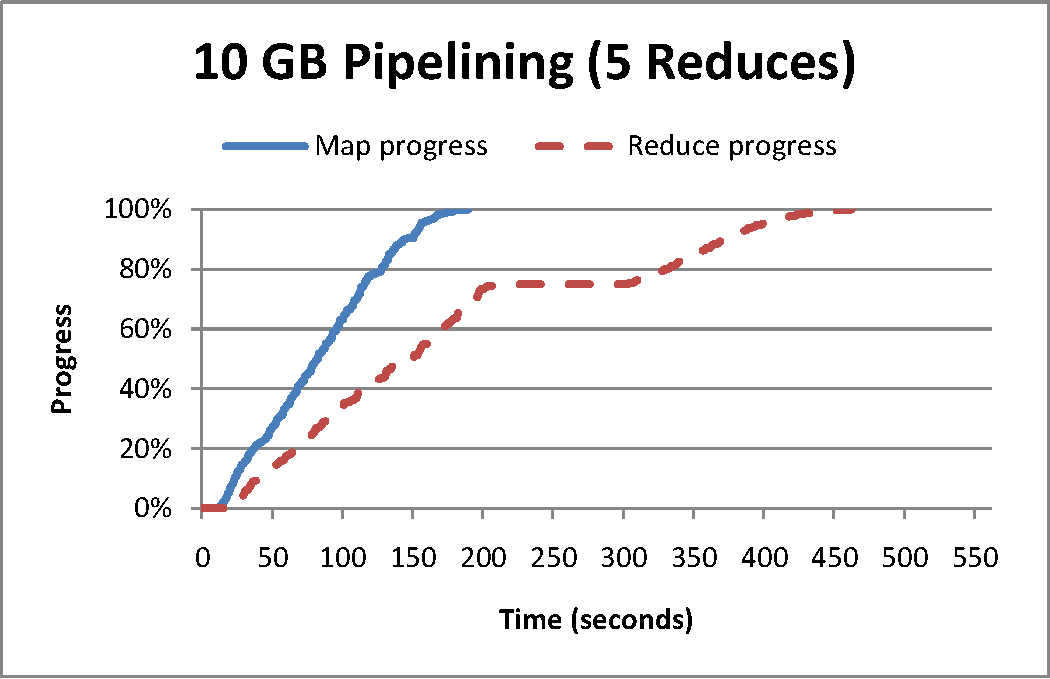
\includegraphics[width=0.95\linewidth]{eval/wc_10gb_20m5r_pipeline}
%\end{minipage}
%\caption{CDF of map and reduce task completion times for a sort job on
%  5.5GB of text extracted from Wikipedia. The total job runtimes were
%  927 seconds for blocking, and 610 seconds for pipelining.}
%\label{fig:sort}
%\end{figure*}

%We conducted a series of performance experiments using a 60-node
%cluster on Amazon EC2. One node executed the Hadoop \JT\ and the HDFS
%\NN, while the remaining 59 nodes served as slaves for running the
%{\TT}s and HDFS {\DN}s. All nodes executed on ``high-CPU medium'' EC2
%instances with 1.7GB of memory and two virtual cores. Each virtual
%core is the equivalent of a 2007-era 2.5Ghz Intel Xeon processor.

%We began by measuring the performance of a simple MapReduce job that
%does not use a combiner. Sorting is commonly used as a benchmark for
%basic MapReduce performance, because of the implicit sort done by the
%reduce phase. We sorted 5.5GB of article text extracted from
%Wikipedia; each word from the text was parsed as a separate
%record. Figure~\ref{fig:sort} describes sort performance on the EC2
%cluster using an HDFS block size of 128MB (yielding 40 map tasks). We
%configured the system to use 59 reducers. In each graph, we give the
%CDF of map and reduce task completion. The left and right graphs
%depict blocking and pipelined performance, respectively.

%Pipelining dominates blocking for this configuration, in part because
%it achieves better cluster utilization: the reduce tasks in the
%blocking job were idle for the first $192$ seconds of the experiment,
%whereas for the pipelined job, reducers began doing useful work within
%$20$ seconds. Note that in a highly-utilized cluster, increased
%pipeline parallelism would not necessarily lead to an improvement in
%total throughput. However, these results suggest that pipelining can
%substantially reduce the response time of an individual job, which can
%often be important (e.g., quickly executing high-priority jobs).
